\documentclass[12pt,a4paper]{article}
\usepackage{ucebnice}
\usepackage{polynom}

\title{Exponenciální funkce}
\author{Ondřej Škubala}
\date{\today}

\begin{document}

\maketitle
\newpage

\section{Exponenciální funkce}


\begin{historicalbox}
Myšlenka exponenciálního růstu se objevovala v lidských dějinách mnohem dříve,
než vznikl samotný pojem exponenciální funkce.
Již starověcí Egypťané a Babyloňané pracovali s úrokováním majetku
a s postupným násobením čísel,
aniž by tyto jevy popisovali pomocí moderní symboliky;
uvědomovali si však, že opakované násobení téhož činitele vede k růstu,
který je mnohem rychlejší než prosté sčítání.
K výraznějšímu matematickému uchopení exponenciálního chování však dochází až ve středověké Evropě,
kdy obchod, finance a účtování začínají vyžadovat přesnější modely.

Zásadní krok učinil John Napier na počátku 17. století,
když představil logaritmy a ukázal, že mnohonásobné násobení lze převést na pouhé sčítání,
což umožnilo astronomům a navigátorům zpracovávat výpočty, které by byly jinak zcela nepřístupné.
Logaritmické tabulky, které tehdy vznikaly, se staly v podstatě prvním „softwarem“ v dějinách matematiky
a zároveň historicky prvním systematickým setkáním lidstva s exponenciální funkcí jakožto hladkou
a dobře popsanou křivkou.

K samotné moderní definici exponenciální funkce vedla práce mnoha matematiků 17. a 18. století,
zejména Leonharda Eulera, jenž ukázal, že funkci $e^{x}$ lze chápat jako limitu rostoucí posloupnosti
a zároveň že tato funkce vystupuje jako řešení celé řady diferenciálních rovnic,
které popisují růst, pohyb či šíření. Eulerovo číslo $e$ se díky tomu stalo jednou
z nejdůležitějších konstant v matematice, neboť představuje přirozenou míru exponenciálního růstu i rozpadu.

Teprve v devatenáctém století se exponenciální funkce usazuje ve školské matematice podobně,
jak ji známe dnes, a stává se základem pro popis finančního úročení, růstu populací,
radioaktivního rozpadu a dalších procesů, v nichž se přírůstky neustále násobí.
Od starověkých úrokových tabulek až po moderní matematické modely tak exponenciální
funkce provází lidstvo více než tři tisíce let,
a přesto její jednoduchá rovnice stále skrývá překvapivé a hluboké vlastnosti.
\end{historicalbox}


V tradiční středoškolské matematice sloužily exponenciální a logaritmické funkce,
stejně jako logaritmy samotné,
především k numerickému výpočtu složitějších příkladů prostřednictvím logaritmických tabulek
nebo logaritmických pravítek, která dokázala převádět násobení a dělení na pouhé sčítání
a tím umožňovala provádět výpočty velmi rychle a s překvapivou přesností.
S nástupem moderních kalkulátorů a počítačů však tato původní praktická funkce logaritmů
ustoupila do pozadí a jejich někdejší role „výpočetního nástroje“ se dnes jeví spíše jako historická zajímavost.

To však v žádném případě neznamená, že by exponenciální a logaritmické funkce ztratily význam ve středoškolské výuce;
naopak, v současném vzdělávání nabývají ještě větší důležitosti než dříve,
a to zejména díky svému přirozenému výskytu v přírodních a technických vědách.
V chemii popisují rychlost radioaktivního rozpadu, reakční kinetiku či poločas přeměny látek,
ve fyzice se objevují při modelování tlumeného kmitání, nabíjení a vybíjení kondenzátorů,
v zeslabení světla nebo v logaritmických akustických stupnicích,
a v biologii vystupují v růstu populací, šíření virů, množení buněk či při popisu metabolismu.
Díky tomu se exponenciální funkce stávají mimořádně mnohostranným tématem,
které propojuje matematiku s reálnými procesy a zároveň ukazuje studentům,
že i zdánlivě jednoduché rovnice mohou popsat překvapivě složité a dynamické děje.



U mocninné funkce, například $y=x^2$, se mění základ mocniny, zatímco exponent zůstává stejný.
Nyní si jejich úlohy vyměníme: základ ponecháme pevný a budeme měnit exponent.
Pro funkci $f(x)=9^x$ tak podle známých pravidel pro mocniny dostáváme
\[
    f(-1)=9^{-1}=\frac19,\qquad
    f(0)=9^0=1,\qquad
    f\left(\frac12\right)=\sqrt9=3,\qquad
    f(1)=9.
\]
Záporný argument tedy neznamená zápornou funkční hodnotu a zlomkový argument nás přirozeně vrací k odmocninám.
Jak jsme již uvedli při rozšiřování mocnin na reálné exponenty, pro kladný základ mají smysl také hodnoty jako $9^{\sqrt2}$;
jejich přibližné hodnoty můžeme určit kalkulačkou.

Chceme-li připustit všechny reálné argumenty, musí být základ kladný.
Nulový základ například neumožňuje dosadit $x=-1$, záporný základ zase $x=\frac12$.
Číslo $1$ sice můžeme umocnit na libovolný reálný exponent, ale vždy dostaneme $1$,
tedy konstantní funkci. Tento případ proto z následující definice vynecháváme.

\begin{definitionbox}
Exponenciální funkcí o základu $a$ nazýváme funkci $f(x)$,
u níž se proměnná $x$ objevuje v exponentu pevného kladného čísla $a\neq1$ a která má tvar
\[
    f(x) = a^{x},\qquad a>0,\quad a\neq1,\quad x\in\mathbb{R}.
\]
\end{definitionbox}

\begin{center}
\begin{minipage}{0.48\textwidth}
\centering
\begin{tikzpicture}[scale=0.85]
    \begin{axis}[
        axis lines=middle,
        xmin=-4, xmax=4,
        ymin=0, ymax=8,
        ticks=none,
        xlabel={$x$}, ylabel={$y$},
        domain=-4:4,
        samples=200,
        smooth,
        title={\small $a>1$ : \quad rostoucí}
    ]
    \addplot[blue, thick] {2^x};
    \addplot[only marks, mark=*] coordinates {(0,1)};
    \node[above left] at (axis cs:0,1) {$[0;1]$};
    \end{axis}
\end{tikzpicture}
\end{minipage}
\hfill
\begin{minipage}{0.48\textwidth}
\centering
\begin{tikzpicture}[scale=0.85]
    \begin{axis}[
        axis lines=middle,
        xmin=-4, xmax=4,
        ymin=0, ymax=8,
        ticks=none,
        xlabel={$x$}, ylabel={$y$},
        domain=-4:4,
        samples=200,
        smooth,
        title={\small $0<a<1$ : \quad klesající}
    ]
    \addplot[red, thick] {(1/2)^x};
    \addplot[only marks, mark=*] coordinates {(0,1)};
    \node[above right] at (axis cs:0,1) {$[0;1]$};
    \end{axis}
\end{tikzpicture}
\end{minipage}
\end{center}

Z uvedených grafů je patrné, že charakter exponenciální funkce je plně určen hodnotou jejího
základu:

\smallskip
Pokud je \textbf{$a>1$}, funkce \important{roste}, neboť každé zvětšení exponentu vede k násobnému
zvětšení její hodnoty a graf se proto prudce zvedá směrem vzhůru.

\smallskip
Naopak při \textbf{$0<a<1$} odpovídá
každý další exponent dalšímu dělení, takže funkce \important{klesá} a její hodnoty se postupně přibližují
k nule, aniž by jí kdy skutečně dosáhly. V obou případech však platí, že exponenciální funkce je vždy
\important{kladná} a nikdy neprotíná osu $x$, která zde vystupuje jako její \textbf{vodorovná asymptota}.

Všechny exponenciální funkce navíc procházejí bodem \textbf{$[0;1]$}, protože libovolné kladné číslo
umocněné na nultou má hodnotu $1$; tento bod tak tvoří společný průsečík všech grafů a představuje
důležitý orientační prvek při jejich srovnávání.



Z definice máme $D(f)=\mathbb{R}$. U kladného základu jsou všechny hodnoty $a^x$ kladné,
ale pro určení oboru hodnot potřebujeme vědět také to, kterých kladných hodnot funkce nabývá.
Pro $a>1$ se při $x\to-\infty$ hodnoty blíží k nule a při $x\to+\infty$ rostou bez omezení;
pro $0<a<1$ jsou oba směry obrácené.
Graf reálné exponenciální funkce je přitom souvislá křivka, mezi jejími hodnotami nevznikají mezery.
Proto nabývá všech kladných hodnot a platí
\[
    H(f)=(0;\infty).
\]

Funkce je tedy omezená zdola, například číslem $0$, ale toto číslo není jejím minimem:
žádný argument nedává hodnotu $a^x=0$.
Ke každé kladné funkční hodnotě navíc existuje jiná, ještě menší kladná hodnota.
Základní exponenciální funkce proto minimum nemá. Není omezená shora, a nemá tedy ani maximum.
Rozdíl mezi dolní závorou a minimem spočívá právě v tom, že minimum musí být skutečně dosaženou funkční hodnotou.

Monotónnost zároveň vysvětluje, proč je exponenciální funkce prostá.
Pro $a>1$ z $x_1<x_2$ plyne $a^{x_1}<a^{x_2}$, zatímco pro $0<a<1$ platí $a^{x_1}>a^{x_2}$.
V obou případech tedy různé argumenty vedou k různým funkčním hodnotám.
Tyto závěry se vztahují k základní funkci $a^x$ na celé $\mathbb{R}$;
u posunutých funkcí nebo při omezení definičního oboru posuzujeme vlastnosti znovu.

\subsection*{Grafy exponenciálních funkcí}
Exponenciální funkce patří mezi nejdůležitější matematické modely, protože
dokonale popisují růst a zánik jevů, jejichž změna probíhá násobením
— nikoli přičítáním. Jejich chování zásadně určuje \textbf{základ exponenciály}:
hodnoty větší než $1$ způsobují rychlý růst, zatímco hodnoty mezi $0$ a $1$
vedou ke stejnoměrně prudkému poklesu. Jemná změna základu často vede k dramaticky
odlišnému průběhu celé funkce, což dobře ilustruje následující společný graf,
kde jsou zobrazeny exponenciální funkce se základy $2$, $5$, $10$ a jejich
„obrácené“ varianty $\left(\frac12\right)^x$, $\left(\frac15\right)^x$ a
$\left(\frac{1}{10}\right)^x$.

\begin{center}
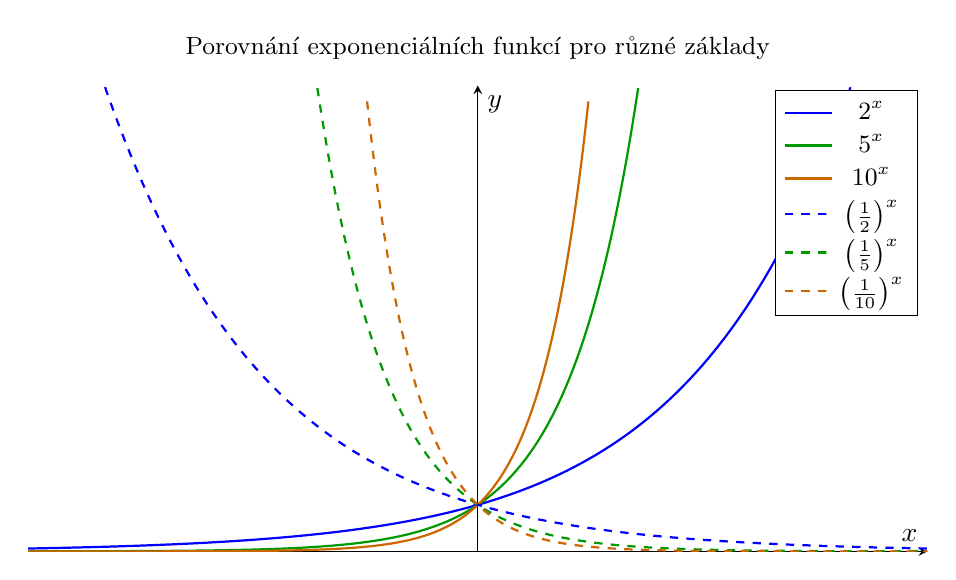
\begin{tikzpicture}[scale=1]
\begin{axis}[
    axis lines=middle,
    xmin=-4, xmax=4,
    ymin=0, ymax=10,
    xlabel={$x$}, ylabel={$y$},
    samples=200,
    legend style={at={(0.99,0.99)}, anchor=north east, font=\small},
    domain=-4:4,
    smooth,
    ticks=none,
    width=13cm, height=7.5cm,
    title={\small Porovnání exponenciálních funkcí pro různé základy},
    restrict y to domain=0:10  % omezí y, aby graf neutekl
]

% ROSTOUCÍ FUNKCE
\addplot[blue, thick] {2^x};
\addlegendentry{$2^x$}

\addplot[green!60!black, thick] {5^x};
\addlegendentry{$5^x$}

\addplot[orange!80!black, thick] {10^x};
\addlegendentry{$10^x$}

% KLESAJÍCÍ FUNKCE
\addplot[blue, thick, dashed] {(1/2)^x};
\addlegendentry{$\left(\frac12\right)^{x}$}

\addplot[green!60!black, thick, dashed] {(1/5)^x};
\addlegendentry{$\left(\frac15\right)^{x}$}

\addplot[orange!80!black, thick, dashed] {(1/10)^x};
\addlegendentry{$\left(\frac{1}{10}\right)^{x}$}

\end{axis}
\end{tikzpicture}
\end{center}


\begin{notebox}
Z grafu je patrné, že čím větší je základ $a>1$, tím rychleji funkce roste.
Naopak základy $0<a<1$ vedou ke klesajícím funkcím, které se pro záporná $x$
prudce zvyšují. Všechny křivky navíc procházejí bodem $[0;1]$.    
\end{notebox}





\begin{samepage}
Význam základu můžeme vystihnout také bez porovnávání strmosti grafů.
Pro základní exponenciální funkci $f(x)=a^x$ využijeme pravidlo pro součin mocnin stejného základu:
\[
    f(x+1)=a^{x+1}=a\cdot a^x=af(x).
\]
\end{samepage}
Zvětšení argumentu o jednu tedy násobí funkční hodnotu stále stejným číslem $a$.
Protože $f(x)>0$, můžeme tento vztah zapsat i jako $\frac{f(x+1)}{f(x)}=a$.
Základ tak udává \textbf{násobný koeficient změny při jednotkovém přírůstku argumentu}.
Jednotkou může být například den nebo kilometr; význam základu proto souvisí i s tím, v jakých jednotkách argument měříme.

Zcela stejně pro libovolná reálná $x$ a $h$ dostaneme
\[
    f(x+h)=a^{x+h}=a^h\cdot a^x=a^h f(x).
\]
Při stejně dlouhých krocích $h$ násobíme hodnoty stejným koeficientem $a^h$.
Neznamená to, že přičítáme stále stejné číslo: absolutní přírůstek závisí na dosavadní hodnotě.
Například základ $1{,}08$ znamená růst o $8\,\%$ za jednotku argumentu,
protože nová hodnota činí $108\,\%$ hodnoty předchozí.
Základ $0{,}92$ naproti tomu znamená pokles o $8\,\%$, neboť zůstává $92\,\%$ předchozí hodnoty.
Při změně o $p\,\%$ používáme pro růst koeficient $1+\frac{p}{100}$
a pro pokles koeficient $1-\frac{p}{100}$, přičemž u poklesu uvažujeme $0<p<100$.

Stejné pravidlo pro mocniny propojuje vodorovný posun grafu s násobením jeho hodnot:
\[
    a^{x+b}=a^b a^x.
\]
Například $5^{x+2}=25\cdot5^x$.
Graf funkce $5^{x+2}$ tedy můžeme získat z grafu $5^x$ buď posunutím o dvě jednotky doleva,
nebo vynásobením všech jeho svislých souřadnic číslem $25$.
Bod $[-2;1]$ prvního popisu leží také na grafu $25\cdot5^x$, neboť $25\cdot5^{-2}=1$.
Jde o různé geometrické úpravy, které zde díky vlastnostem mocnin vedou ke stejné výsledné funkci.

\section*{Sestavování grafu exponenciální funkce}

Při sestavování grafů je užitečné vycházet ze základní exponenciální funkce $y=a^{x}$,
jejíž graf následně posouváme, protahujeme nebo jinak modifikujeme pomocí jednoduchých úprav
v exponentu či mimo něj.

Důležitým bodem základní exponenciální funkce $y=a^x$ je bod \textbf{$[0;1]$}, který slouží jako hlavní orientační prvek.
Nahrazení $x$ výrazem $x+b$ posouvá tento bod po ose $x$,
zatímco přičtení konstanty $c$ mimo exponenciálu posouvá celý graf svisle po ose $y$.
Stejným způsobem se posouvá i vodorovná asymptota, která u funkce $a^{x}$ leží na ose $x$
a u funkcí typu $a^{x}+c$ nebo $a^{x+b}+c$ se posouvá na výšku $y=c$.

Při sestavování grafů funkcí tvaru $f(x)=a^{x+b}+c$ tedy postupujeme ve dvou jednoduchých krocích:
nejprve provedeme vodorovný posun o $-b$ a následně svislý posun o $c$.
Touto metodou lze sestavit grafy těchto funkcí, aniž bychom potřebovali tabulku hodnot.
Násobení funkčních hodnot koeficientem $m$ ve funkci $m\cdot a^x$ mění svislé měřítko grafu a pro $m<0$ jej navíc převrací podle osy $x$.
Nahrazení $x$ výrazem $kx$ pro $k\neq0$ mění vodorovné měřítko a pro $k<0$ přidává souměrnost podle osy $y$.



\begin{examplebox}{Sestavení grafu funkce $f(x)=2^{x+3}-4$}

\textbf{1. Výchozí funkce: $y=2^{x}$}

Tato funkce prochází bodem $[0;1]$ a má vodorovnou asymptotu $y=0$.
Je rostoucí, protože základ $2$ je větší než jedna.

\begin{center}
\begin{tikzpicture}[scale=0.85]
    \begin{axis}[
        axis lines=middle,
        xmin=-5, xmax=3,
        ymin=-1, ymax=8,
        ticks=none,
        xlabel={$x$}, ylabel={$y$},
        domain=-5:3,
        samples=200,
        smooth,
        title={\small Výchozí funkce $2^{x}$}
    ]
    \addplot[blue, thick] {2^x};
    \addplot[only marks, mark=*] coordinates {(0,1)};
    \node[above left] at (axis cs:0,1) {$[0;1]$};
    \draw[dashed] (axis cs:-5,0) -- (axis cs:3,0);
    \node[below] at (axis cs:-4,0) {$y=0$};
    \end{axis}
\end{tikzpicture}
\end{center}



\textbf{2. Posun po ose $x$: $y=2^{x+3}$}

Výraz \,$x+3$ znamená posun \textbf{o tři jednotky doleva},
protože funkční argument se zvětšuje rychleji, než původně.
Bod $[0;1]$ se tedy posune na souřadnice $[-3;1]$.
Asymptota zůstává stále na $y=0$.

\begin{center}
\begin{tikzpicture}[scale=0.85]
    \begin{axis}[
        axis lines=middle,
        xmin=-8, xmax=0,
        ymin=-1, ymax=8,
        ticks=none,
        xlabel={$x$}, ylabel={$y$},
        domain=-8:0,
        samples=200,
        smooth,
        title={\small Posun vlevo: $2^{x+3}$}
    ]
    % Funkce
    \addplot[blue, thick] {2^(x+3)};

    % Bod
    \addplot[only marks, mark=*] coordinates {(-3,1)};
    \node[above left] at (axis cs:-3,1) {$[-3;1]$};

    % Pomocné čáry k osám
    \draw[dashed] (axis cs:-3,1) -- (axis cs:-3,0);   % k ose x
    \draw[dashed] (axis cs:-3,1) -- (axis cs:0,1);    % k ose y

    % Asymptota
    \draw[dashed] (axis cs:-8,0) -- (axis cs:0,0);
    \node[below] at (axis cs:-7,0) {$y=0$};
    \end{axis}
\end{tikzpicture}
\end{center}




\textbf{3. Posun po ose $y$: $y=2^{x+3}-4$}

Hodnota $-4$ posouvá celou křivku o čtyři jednotky dolů.
Bod $[-3;1]$ se posune na $[-3;-3]$.
Vodorovná asymptota se posouvá z $y=0$ na \textbf{$y=-4$}.

\begin{center}
\begin{tikzpicture}[scale=0.85]
    \begin{axis}[
        axis lines=middle,
        xmin=-8, xmax=0,
        ymin=-8, ymax=4,
        ticks=none,
        xlabel={$x$}, ylabel={$y$},
        domain=-8:0,
        samples=200,
        smooth,
        title={\small Posun dolů: $2^{x+3}-4$}
    ]
    % Funkce
    \addplot[blue, thick] {2^(x+3)-4};

    % Bod
    \addplot[only marks, mark=*] coordinates {(-3,-3)};
    \node[above left] at (axis cs:-3,-3) {$[-3;-3]$};

    % Pomocné čáry
    \draw[dashed] (axis cs:-3,-3) -- (axis cs:-3,0);   % svislá k ose x
    \draw[dashed] (axis cs:-3,-3) -- (axis cs:0,-3);   % vodorovná k ose y

    % Asymptota
    \draw[dashed] (axis cs:-8,-4) -- (axis cs:0,-4);
    \node[below] at (axis cs:-7,-4) {$y=-4$};

    \end{axis}
\end{tikzpicture}
\end{center}


Tímto postupem snadno sestavíme celý graf, aniž bychom potřebovali vypisovat tabulku hodnot.
Stačí sledovat, jak jednotlivé úpravy posouvají výchozí exponenciální křivku.
Z výsledného předpisu můžeme určit i další vlastnosti funkce.
Exponent $x+3$ má smysl pro každé reálné $x$, proto $D(f)=\mathbb{R}$.
Výraz $2^{x+3}$ nabývá všech kladných hodnot a odečtením čtyř dostaneme $H(f)=(-4;\infty)$.
Funkce zůstává rostoucí; posuny tuto vlastnost nemění.
Hodnota $-4$ je dolní závorou, ale není dosažena, takže funkce minimum nemá.

Průsečík s osou $y$ získáme dosazením $x=0$: $f(0)=2^3-4=4$, tedy $P_y=[0;4]$.
Pro průsečík s osou $x$ potřebujeme nulovou funkční hodnotu.
Protože $2^2=4$, vyhovuje $x+3=2$, tedy $x=-1$.
Dosazení $f(-1)=2^2-4=0$ potvrzuje bod $P_x=[-1;0]$;
jiný průsečík s osou $x$ neexistuje, protože funkce je rostoucí.

\end{examplebox}


\begin{notebox}
\textbf{Asymptota} je přímka, od níž se vzdálenost bodů na neomezené větvi grafu blíží k nule.
Graf se může asymptoty dotknout nebo ji protnout.
U základní exponenciální funkce však graf osu $x$ neprotíná,
protože všechny její funkční hodnoty jsou kladné.

\begin{itemize}
    \item \textbf{Svislá asymptota} vzniká tehdy, když se funkce blíží k $\pm\infty$ 
    při přibližování k určité hodnotě $x$ alespoň z jedné strany.  
    Například u logaritmu $y = \log_2 x$ je svislou asymptotou přímka \important{$x = 0$}.

    \item \textbf{Vodorovná asymptota} $y=c$ vzniká tehdy, když se rozdíl $f(x)-c$
    blíží k nule při $x\to+\infty$ nebo $x\to-\infty$.  
    Například exponenciála $y = 2^{-x}$ má vodorovnou asymptotu \important{$y = 0$}.
\end{itemize}

Asymptoty pomáhají pochopit, jak se funkce chová „daleko od středu grafu“ 
a ke kterým přímkám se jeho neomezené větve přibližují.
\end{notebox}


\begin{examplebox}{Sestavení grafu funkce $g(x)=-2\cdot2^x+3$}

Sestrojíme graf a určíme jeho základní vlastnosti.
Vycházíme opět z funkce $y=2^x$, ale tentokrát kromě posunu použijeme také násobení funkčních hodnot.

Nejprve přejdeme k funkci $y=2\cdot2^x$.
Každá svislá souřadnice se zdvojnásobí, zatímco vodorovná souřadnice zůstane stejná.
Například bod $[0;1]$ přejde na $[0;2]$.
Znaménko minus pak graf převrátí podle osy $x$:
u funkce $y=-2\cdot2^x$ získáme bod $[0;-2]$.
Nakonec přičteme $3$, tedy celý graf posuneme o tři jednotky nahoru.
Výsledný charakteristický bod je $[0;1]$ a vodorovná asymptota se posune z $y=0$ na $y=3$.

Stejným způsobem se každý bod $[u;2^u]$ základního grafu změní na $[u;-2\cdot2^u+3]$.
Několik bodů ověříme přímo dosazením do výsledného předpisu:
\[
\begin{aligned}
g(-1)&=-2\cdot\frac12+3=2, & g(0)&=-2\cdot1+3=1,\\
g(1)&=-2\cdot2+3=-1, & g(2)&=-2\cdot4+3=-5.
\end{aligned}
\]
Tyto body umožňují zkontrolovat, zda jsme správně provedli násobení, převrácení i posun.

\begin{center}
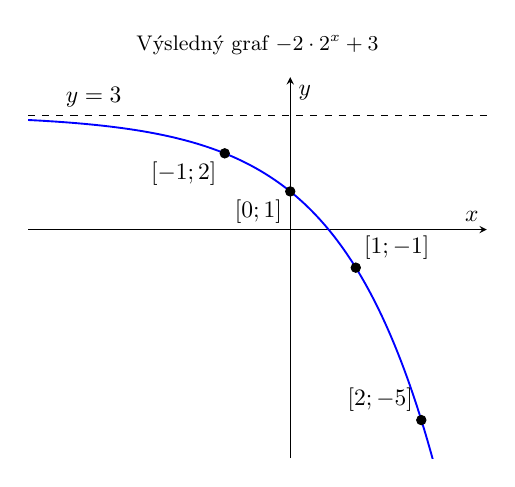
\begin{tikzpicture}[scale=0.85]
    \begin{axis}[
        axis lines=middle,
        xmin=-4, xmax=3,
        ymin=-6, ymax=4,
        ticks=none,
        xlabel={$x$}, ylabel={$y$},
        domain=-4:3,
        samples=200,
        smooth,
        title={\small Výsledný graf $-2\cdot2^x+3$}
    ]
    \addplot[blue, thick] {-2*2^x+3};
    \addplot[only marks, mark=*] coordinates {(-1,2) (0,1) (1,-1) (2,-5)};
    \node[below left] at (axis cs:-1,2) {$[-1;2]$};
    \node[below left] at (axis cs:0,1) {$[0;1]$};
    \node[above right] at (axis cs:1,-1) {$[1;-1]$};
    \node[above left] at (axis cs:2,-5) {$[2;-5]$};
    \draw[dashed] (axis cs:-4,3) -- (axis cs:3,3);
    \node[above] at (axis cs:-3,3) {$y=3$};
    \end{axis}
\end{tikzpicture}
\end{center}

Funkce $2^x$ je rostoucí, ale násobení záporným číslem $-2$ obrátí pořadí jejích hodnot.
Přičtení trojky už pořadí nezmění, takže $g$ je na celé $\mathbb{R}$ \textbf{klesající}.
Definiční obor zůstává $D(g)=\mathbb{R}$.
Z kladnosti $2^x$ plyne $-2\cdot2^x+3<3$ a všechny hodnoty menší než $3$ jsou dosaženy.
Proto
\[
    H(g)=(-\infty;3).
\]
Při $x\to-\infty$ se $2^x$ blíží k nule, a rozdíl $g(x)-3=-2\cdot2^x$ se tedy blíží k nule také.
Vodorovnou asymptotou je $y=3$; graf k ní přichází zdola a nedosáhne jí.
Při $x\to+\infty$ funkční hodnoty klesají bez omezení.
\end{examplebox}

\subsection*{Exponenciální růst vs.\ mocninný růst}

Přestože se může zdát, že funkce $x^{n}$ roste velmi rychle, zejména pro vysoké hodnoty exponentu $n$,
její tempo růstu je i tak nesrovnatelně pomalejší než u exponenciálních funkcí $a^{x}$.
Mocninný růst znamená, že při každém zvětšení $x$ se hodnota násobí určitou
silou proměnné, zatímco exponenciální růst znamená, že se násobí \emph{stále stejným číslem}
v každém kroku. Z toho vyplývá zásadní rozdíl: zatímco $x^{n}$ se stává velkým až pro opravdu
vysoké hodnoty $x$, funkce $a^{x}$ se po překročení určité hranice začne „utrhávat“
a roste tak rychle, že libovolnou mocninu nejen dožene, ale ve velmi krátkém čase i dramaticky předhoní.

Tento fakt je natolik obecný, že v matematice platí důležité tvrzení:
\emph{každá exponenciální funkce $a^{x}$ s $a>1$ nakonec převýší libovolnou mocninnou funkci $x^{n}$}.

\bigskip
\begin{center}
    \begin{tabular}{c|c|c|c|c}
    $x$ & $x^{3}$ & $2^{x}$ & $x^{10}$ & $10^{x}$ \\
    \hline
    2           & 8                     & 4                         & 1024                      & 100 \\
    5           & 125                   & 32                        & 9\,765\,625               & 100\,000 \\
    10          & 1000                  & 1024                      & 10\,000\,000\,000         & 10\,000\,000\,000 \\
    20          & 8000                  & 1\,048\,576               & $10^{13}$                 & $10^{20}$ \\
    50          & 125\,000              & 1.13 $\cdot 10^{15}$      & $10^{17}$                 & $10^{50}$ \\
    100         & 1\,000\,000           & 1.27 $\cdot 10^{30}$      & $10^{20}$                 & $10^{100}$ \\
    500         & 125\,000\,000         & 3.27 $\cdot 10^{150}$     & 9.77 $\cdot 10^{26}$      & $10^{500}$ \\
    1000        & 1 $\cdot 10^{9}$      & 1.07 $\cdot 10^{301}$     & 1 $\cdot 10^{30}$         & $10^{1000}$ \\
    2000        & 8 $\cdot 10^{9}$      & 1.15 $\cdot 10^{602}$     & 1.02 $\cdot 10^{33} $     & $10^{2000}$ \\
    \end{tabular}
\end{center}

\bigskip
\begin{notebox}{Srovnání růstu: $x^{10}$ vs.\ $2^{x}$}
Při malých hodnotách proměnné $x$ se může zdát, že funkce $x^{10}$ roste rychleji než $2^{x}$,
protože již pro $x=5$ má hodnotu téměř deseti milionů, zatímco $2^{5}=32$.
Jakmile však $x$ začne narůstat, exponenciála začíná dominovat: již kolem $x=50$
platí, že $2^{50}$ je přibližně $10^{15}$, zatímco $50^{10}$ je přibližně $10^{17}$,
a krátce poté funkce $2^{x}$ nejen dožene, ale i dramaticky předstihne každou mocninu $x^{n}$.
To ukazuje, že exponenciální růst je kvalitativně odlišný od mocninného a vede k hodnotám,
jež rychle přesahují běžnou představivost.
\end{notebox}

\bigskip
\begin{examplebox}{Sestavení grafu funkce $y = \big|\,2^{x-2} - 4\,\big|$}

Budeme postupovat ve čtyřech krocích, přičemž pokaždé sledujeme,
jak se mění výchozí exponenciální křivka, její charakteristický bod
a vodorovná asymptota. Teprve poté aplikujeme absolutní hodnotu,
která část grafu překlopí nad osu $x$.
% ============================================================
% 1. KROK – y = 2^x
% ============================================================

\textbf{1. Výchozí funkce: $y=2^{x}$}

Funkce je rostoucí, prochází bodem $[0;1]$ a její asymptota je $y=0$.

\begin{center}
\begin{tikzpicture}[scale=0.95]
\begin{axis}[
    axis lines=middle,
    xmin=-10, xmax=10,
    ymin=-10, ymax=10,
    ticks=none,
    xlabel={$x$}, ylabel={$y$},
    domain=-10:10,
    samples=200,
    smooth,
    title={\small Výchozí funkce $2^{x}$}
]
\addplot[blue, thick] {2^x};

\addplot[only marks, mark=*] coordinates {(0,1)};
\node[above left] at (axis cs:0,1) {$[0;1]$};

\draw[dashed] (axis cs:0,1) -- (axis cs:0,0);
\draw[dashed] (axis cs:0,1) -- (axis cs:0,1);

\draw[dashed] (axis cs:-10,0) -- (axis cs:10,0);
\node[below] at (axis cs:-8,0) {$y=0$};
\end{axis}
\end{tikzpicture}
\end{center}

% ============================================================
% 2. KROK – y = 2^(x-2)
% ============================================================

\textbf{2. Posun doprava o 2: $y=2^{x-2}$}

Bod $[0;1]$ se posune na $[2;1]$, asymptota zůstává na $y=0$.

\begin{center}
\begin{tikzpicture}[scale=0.95]
\begin{axis}[
    axis lines=middle,
    xmin=-10, xmax=10,
    ymin=-10, ymax=10,
    ticks=none,
    xlabel={$x$}, ylabel={$y$},
    domain=-10:10,
    samples=200,
    smooth,
    title={\small Posun doprava: $2^{x-2}$}
]
\addplot[blue, thick] {2^(x-2)};

\addplot[only marks, mark=*] coordinates {(2,1)};
\node[above left] at (axis cs:2,1) {$[2;1]$};

\draw[dashed] (axis cs:2,1) -- (axis cs:2,0);
\draw[dashed] (axis cs:2,1) -- (axis cs:0,1);

\draw[dashed] (axis cs:-10,0) -- (axis cs:10,0);
\node[below] at (axis cs:-8,0) {$y=0$};
\end{axis}
\end{tikzpicture}
\end{center}

% ============================================================
% 3. KROK – y = 2^(x-2) - 4
% ============================================================

\textbf{3. Posun dolů o 4: $y=2^{x-2} - 4$}

Bod $[2;1]$ se posune na $[2;-3]$.
Asymptota klesne na $y=-4$.

\begin{center}
\begin{tikzpicture}[scale=0.95]
\begin{axis}[
    axis lines=middle,
    xmin=-10, xmax=10,
    ymin=-10, ymax=10,
    ticks=none,
    xlabel={$x$}, ylabel={$y$},
    domain=-10:10,
    samples=200,
    smooth,
    title={\small Posun dolů: $2^{x-2}-4$}
]
\addplot[blue, thick] {2^(x-2)-4};

\addplot[only marks, mark=*] coordinates {(2,-3)};
\node[above left] at (axis cs:2,-3) {$[2;-3]$};

\draw[dashed] (axis cs:2,-3) -- (axis cs:2,0);
\draw[dashed] (axis cs:2,-3) -- (axis cs:0,-3);

\draw[dashed] (axis cs:-10,-4) -- (axis cs:10,-4);
\node[below] at (axis cs:-8,-4) {$y=-4$};
\end{axis}
\end{tikzpicture}
\end{center}

% ============================================================
% 4. KROK – y = |2^(x-2) - 4|
% ============================================================

\textbf{4. Absolutní hodnota: $y=\big|\,2^{x-2}-4\,\big|$}

Část pod osou $x$ se odrazí nahoru. Původní funkce nemá minimum;
hodnota $-4$ určuje pouze její vodorovnou asymptotu při $x\to-\infty$.
Výsledná funkce má minimum $0$ v bodě $[4;0]$, obor hodnot $[0;\infty)$
a vodorovnou asymptotu $y=4$ při $x\to-\infty$.

\begin{center}
\begin{tikzpicture}[scale=0.95]
\begin{axis}[
    axis lines=middle,
    xmin=-10, xmax=10,
    ymin=-10, ymax=10,
    ticks=none,
    xlabel={$x$}, ylabel={$y$},
    domain=-10:10,
    samples=400,
    smooth,
    title={\small Absolutní hodnota: $|2^{x-2}-4|$}
]
\addplot[blue, thick] {abs(2^(x-2)-4)};

% nový bod (odraz)
\addplot[only marks, mark=*] coordinates {(2,3)};
\node[above left] at (axis cs:2,3) {$[2;3]$};

\draw[dashed] (axis cs:2,3) -- (axis cs:2,0);
\draw[dashed] (axis cs:2,3) -- (axis cs:0,3);

\end{axis}
\end{tikzpicture}
\end{center}

Tímto postupem lze sestrojit graf i složitě vypadajících funkcí,
pokud úpravy provádíme postupně a sledujeme změny v exponentu
a mimo exponent samostatně.
\end{examplebox}


\subsection*{Využití grafu exponenciální funkce k určování hodnot}
Exponenciální funkce je velmi rychle rostoucí nebo klesající křivka, jejíž tvar je natolik
pravidelný, že nám v mnoha případech umožňuje odhadnout či porovnat hodnoty výrazů,
aniž bychom museli provádět přesné numerické výpočty. Zvláště v situacích,
kdy se hodnoty exponentů liší jen nepatrně, může být numerické srovnání obtížné
a někdy i nepraktické, zatímco pohled na graf funkce $a^{x}$ poskytne okamžitou
odpověď. Pokud víme, zda je exponenciální funkce \important{rostoucí} nebo \important{klesající},
stačí určit, ve kterém z těchto případů se nacházíme, a podle toho vyvodit,
který z porovnávaných výrazů je větší. Graf tak přestává být pouze ilustrací,
ale stává se účinným nástrojem pro rozhodování o velikosti hodnot,
jež by se jinak obtížně porovnávaly.

\begin{examplebox}{Porovnání výrazů $\,(0{,}4)^{1{,}6}$ a $\,(0{,}4)^{1{,}8}$}

Nejprve si všimneme, že základ $0{,}4$ splňuje $0 < 0{,}4 < 1$.
Exponenciální funkce s takovým základem je \important{klesající},
což znamená, že větší hodnota exponentu vede k menší hodnotě celého výrazu.

\medskip
\textbf{1. Porovnání početním způsobem}

Základ je stejný, exponenty se liší jen nepatrně:

\[
1{,}6 < 1{,}8.
\]

Protože je funkce $f(x)=0{,}4^{x}$ klesající, platí:

\[
(0{,}4)^{1{,}6} > (0{,}4)^{1{,}8}.
\]

Výsledek dostaneme okamžitě, bez počítání hodnot.

\medskip
\textbf{2. Porovnání pomocí grafu}

Nyní se podíváme na graf funkce $y = 0{,}4^{x}$:

\begin{center}
\begin{tikzpicture}[scale=1]
\begin{axis}[
    axis lines=middle,
    xmin=0, xmax=3,
    ymin=0, ymax=1.2,
    xlabel={$x$}, ylabel={$y$},
    samples=300,
    smooth,
    ticks=none,
    title={\small Graf funkce $0{,}4^{x}$}
]

% hlavní křivka
\addplot[blue, thick] {(0.4)^x};

% numerické hodnoty bodů
\addplot[only marks, mark=*] coordinates {(1.6, 0.23)};
\addplot[only marks, mark=*] coordinates {(1.8, 0.192)};

% popisky bodů
\node[right] at (axis cs:1.6, 0.263) {$x=1{,}6$};
\node[right] at (axis cs:1.8, 0.192) {$x=1{,}8$};

% pomocné čáry
\draw[dashed] (axis cs:1.6,0) -- (axis cs:1.6,0.230832);
\draw[dashed] (axis cs:1.8,0) -- (axis cs:1.8,0.192);

\end{axis}
\end{tikzpicture}
\end{center}


Z grafu ihned vidíme, že $0{,}4^{x}$ je klesající křivka:
bod odpovídající $x=1{,}6$ leží \textbf{výše} než bod pro $x=1{,}8$,
což potvrzuje předchozí závěr.

\medskip

\textbf{Závěr:}

\[
(0{,}4)^{1{,}6} > (0{,}4)^{1{,}8}
\]

Grafické porovnání je velmi přehledné a zejména u klesajících exponenciál rychle ukáže,
který exponent vede k větší hodnotě.
\end{examplebox}



\begin{examplebox}{Určení parametrů funkce ze dvou bodů}

Určete parametry $m,c$ tak, aby graf funkce $y=m\cdot2^x+c$
procházel body $A[0;5]$ a $B[2;17]$.

Souřadnice každého bodu na grafu musí splňovat předpis funkce.
Z bodu $A$ tedy dosadíme současně $x=0$ a $y=5$;
z bodu $B$ dosadíme $x=2$ a $y=17$.
Základ exponenciály je zadaný, neznáme pouze její násobný koeficient a svislý posun.
Dostáváme dvě podmínky
\[
    5=m\cdot2^0+c=m+c,\qquad
    17=m\cdot2^2+c=4m+c,
\]
tedy soustavu
\[
\begin{aligned}
    m+c&=5,\\
    4m+c&=17.
\end{aligned}
\]
Odečtením první rovnice od druhé se zbavíme $c$:
$3m=12$, a proto $m=4$.
Dosazením do první rovnice získáme $4+c=5$, tedy $c=1$.
Oba parametry jsou určeny jednoznačně a výsledná funkce má předpis
\[
    y=4\cdot2^x+1.
\]

Výsledek zkontrolujeme v původních bodech:
pro $x=0$ dostaneme $4\cdot1+1=5$, pro $x=2$ vyjde $4\cdot4+1=17$.
Graf tedy skutečně prochází oběma zadanými body.

Protože $4=2^2$, můžeme výsledek zapsat také jako
\[
    4\cdot2^x+1=2^2\cdot2^x+1=2^{x+2}+1.
\]
Tentýž graf tak získáme i posunutím základního grafu $2^x$ o dvě jednotky doleva a o jednu nahoru.
\end{examplebox}

\begin{examplebox}{Monotónnost exponenciální funkce s parametrem}

Určete, pro které hodnoty reálného parametru $q$ je předpis
\[
    f_q(x)=\left(\frac{q^2-9}{q-3}\right)^x
\]
exponenciální funkcí na celé $\mathbb{R}$, a rozhodněte, kdy je tato funkce rostoucí a kdy klesající.

Nejprve potřebujeme, aby byl základ vůbec definovaný.
Ze jmenovatele dostáváme podmínku $q\neq3$.
Teprve s touto podmínkou rozložíme čitatel a zkrátíme:
\[
    \frac{q^2-9}{q-3}
    =\frac{(q-3)(q+3)}{q-3}
    =q+3,\qquad q\neq3.
\]
Krácení znamená dělení nenulovým výrazem, proto původní podmínka nezmizí.
Při $q=3$ bychom do původního základu dosadili zlomek $\frac00$, který nemá smysl;
samotný výraz $q+3$ tuto informaci již neobsahuje.

Základ exponenciální funkce musí být kladný a různý od jedné.
Proto dále požadujeme
\[
    q+3>0,\qquad q+3\neq1,
\]
tedy $q>-3$ a $q\neq-2$.
Spolu s původní podmínkou $q\neq3$ tak získáme všechny přípustné hodnoty
\[
    q\in(-3;-2)\cup(-2;3)\cup(3;\infty).
\]
Pro $q=-3$ je základ nulový a předpis nelze vyhodnotit pro všechna reálná $x$.
Při $q<-3$ je základ záporný, takže například mocnina s exponentem $\frac12$ nemá reálnou hodnotu.
Při $q=-2$ sice vznikne funkce $1^x=1$, ale ta je konstantní a podle naší definice není exponenciální.

Nyní stačí porovnat přípustný základ s jedničkou.
Rostoucí funkci dostaneme právě tehdy, když $q+3>1$, tedy $q>-2$.
Stále ovšem musíme vyloučit $q=3$, takže
\[
    \text{rostoucí pro }q\in(-2;3)\cup(3;\infty).
\]
Klesající funkce vyžaduje $0<q+3<1$, což je ekvivalentní podmínce $-3<q<-2$:
\[
    \text{klesající pro }q\in(-3;-2).
\]
Například pro $q=0$ dostaneme rostoucí funkci $3^x$,
zatímco pro $q=-\frac52$ dostaneme klesající funkci $\left(\frac12\right)^x$.
Podmínky řešíme pro parametr $q$; argument $x$ přitom může nabývat všech reálných hodnot.
\end{examplebox}

\begin{examplebox}{Sestavení exponenciálního modelu}

Na začátku pokusu má porost plochu $80\,\mathrm{cm}^2$.
Podle zvoleného modelu se jeho plocha každé dvě hodiny zvětší o $25\,\%$.
Sestavte předpis funkce $A(t)$, která udává plochu porostu po $t$ hodinách,
a ověřte jej pro několik hodnot času.
Než budete pokračovat ve čtení, zkuste si zapsat plochu na začátku pokusu a po prvních dvou časových intervalech.

Čas začínáme měřit při zahájení pokusu, proto $t=0$ a $A(0)=80$.
Zvětšení o $25\,\%$ znamená, že po každých dvou hodinách zůstává původní plocha
a přibude ještě její čtvrtina:
\[
    A(2)=80+\frac{25}{100}\cdot80
        =80\cdot1{,}25=100.
\]
V dalším dvouhodinovém intervalu počítáme čtvrtinu z aktuálních $100\,\mathrm{cm}^2$,
nikoli z počátečních osmdesáti.
Proto
\[
    A(4)=100\cdot1{,}25
        =80\cdot1{,}25^2=125.
\]
Násobný koeficient zůstává stejný, ale absolutní přírůstky stejné nejsou:
v prvním intervalu přibylo $20\,\mathrm{cm}^2$, ve druhém $25\,\mathrm{cm}^2$.

Po $n$ celých dvouhodinových intervalech tedy dostaneme plochu $80\cdot1{,}25^n$.
Pokud čas vyjadřujeme v hodinách, počet těchto intervalů je $\frac{t}{2}$.
Přijmeme-li exponenciální průběh také mezi jejich konci, získáme předpis
\[
    A(t)=80\cdot1{,}25^{t/2},\qquad t\geq0.
\]
Hodnotu $A(t)$ v tomto zápisu vyjadřujeme v $\mathrm{cm}^2$ a $t$ je číselná hodnota času v hodinách.
Koeficient $1{,}25$ patří ke dvěma hodinám, proto nesmíme při tomto významu $t$ použít exponent $t$.
Poměr $\frac{t}{2}$ vyjadřuje podíl času a délky intervalu měřených ve stejné jednotce.
Kdybychom místo toho použili číselnou hodnotu času $s$ v minutách, zapsali bychom stejný model jako $80\cdot1{,}25^{s/120}$.

Předpis ověříme dosazením:
\[
\begin{aligned}
    A(0)&=80\cdot1{,}25^0=80, &
    A(2)&=80\cdot1{,}25^1=100,\\
    A(4)&=80\cdot1{,}25^2=125, &
    A(6)&=80\cdot1{,}25^3=156{,}25.
\end{aligned}
\]
Po jedné hodině model předpovídá
$A(1)=80\sqrt{1{,}25}\approx89{,}44\,\mathrm{cm}^2$.
Odmocnina odpovídá polovině dvouhodinového intervalu.

Předpokládáme, že při stejných podmínkách zůstává násobný koeficient růstu stejný.
Údaje na koncích dvouhodinových intervalů samy o sobě neurčují průběh mezi nimi;
právě exponenciální průběh jsme zde zvolili jako součást modelu.
V reálném porostu může růst později omezit prostor, dostupnost živin nebo změna prostředí.
Předpis proto používáme jen po dobu, kdy je předpoklad stejného koeficientu přiměřený;
není tvrzením o neomezeném skutečném růstu.
Stejnou úvahu o počtu intervalů využijeme i při exponenciálním poklesu,
kde je násobný koeficient mezi nulou a jedničkou.
\end{examplebox}

% -----------------------------------------------------------------
% ---------------------- P Ř Í K L A D Y --------------------------
% -----------------------------------------------------------------

\exercisepart
\setcounter{section}{1}

% =========================
% ÚLOHA 1 – Kvadratické rovnice k procvičení
% =========================
\begin{exercise}[Určení základního tvaru]
U každé z následujících funkcí určete, zda je rostoucí či klesající,
zapište její základní tvar $m\cdot a^{x+k}+c$ (pokud je vhodné)
a načrtněte její graf.

\begin{tasks}(2)
    \task $y = 2^{x}$
    \task $y = 2^{3x}$
    \task $y = 3^{-x} - 1$
    \task $y = \left(\dfrac12\right)^{2x}$
    \task $y = 2^{x+1} - 4$
    \task $y = \left(\dfrac13\right)^{-2x}$
    \task $y = 2^{x}\cdot 3^{-x}$
    \task $y = 5 \cdot 4^{x-1}$
    \task $y = 7^{\,2-x}$
    \task $y = \left(\dfrac{1}{6}\right)^{-x+1} - 1$
    \task $y = 5^{-x} + 2$
    \task $y = 10^{\,2x + 5} + 8$
    \task $y = 9^{0{,}5x}\cdot 3 + 2$
    \task $y = 16^{-0{,}25x}$
\end{tasks}
\end{exercise}


% =========================
% ÚLOHA 2 – Porovnání s číslem 1
% =========================
\begin{exercise}[Porovnání hodnot exponenciálních výrazů s číslem 1]
Na základě vlastností exponenciální funkce rozhodněte,
zda je uvedená hodnota \textbf{větší než 1}, \textbf{menší než 1},
nebo se jí \textbf{rovná}.
Nepočívejte přesnou hodnotu, rozhodněte pouze podle základu a exponentu.

\begin{tasks}(4)
    \task $\left(\dfrac{2}{5}\right)^{\frac34}$
    \task $\left(\dfrac{5}{4}\right)^{\frac37}$
    \task $2{,}18^{\,0{,}1}$
    \task $0{,}45^{\,0{,}4}$
    \task $\left(\dfrac{41}{40}\right)^{0{,}2}$
    \task $\left(\dfrac{\pi}{4}\right)^{\sqrt{1{,}001}}$
    \task $\left(\dfrac{\pi + 1}{4}\right)^{-2}$
    \task $\left(\dfrac{3}{8}\right)^{\sqrt{2}}$
\end{tasks}
\end{exercise}


% =========================
% ÚLOHA 3 – Pravdivost výroků o mocninách
% =========================
\begin{exercise}[Pravdivost výroků – vlastnosti exponenciálních funkcí]
Rozhodněte, zda jsou následující tvrzení \textbf{pravdivá}, nebo \textbf{nepravdivá}.

\begin{tasks}(2)
    \task $\left(\frac{6}{7}\right)^{2{,}5} < \left(\frac{6}{7}\right)^{2{,}4}$
    \task $\left(\frac{4}{3}\right)^{1{,}4} < \left(\frac{4}{3}\right)^{1{,}3}$
    \task $\left(\frac{1}{5}\right)^{-3} > \left(\frac{1}{5}\right)^{-2}$
    \task $3^{-0{,}8} > 3^{-1{,}1}$
    \task $\left(\frac{9}{10}\right)^{\sqrt{2}} > \left(\frac{9}{10}\right)^{1{,}3}$
    \task $2^{\pi} > 2^{3}$
    \task $\left(\frac{5}{2}\right)^{-0{,}5} < \left(\frac{5}{2}\right)^{-1}$
    \task $\left(\frac{3}{4}\right)^{0{,}01} = \left(\frac{16}{9}\right)^{-\frac{1}{50}}$
\end{tasks}
\end{exercise}


% =========================
% ÚLOHA 4 – Vztah mezi exponenty p a r
% =========================
\begin{exercise}[Vztah mezi exponenty $p$ a $r$]
Rozhodněte, jaký vztah ($p<r$, $p>r$, $p=r$) platí mezi čísly $p$ a $r$,
jestliže platí daná nerovnost. Nepočítejte konkrétní hodnoty, využijte pouze
monotónnost exponenciálních funkcí.

\begin{tasks}(2)
    \task $\left(\dfrac{3}{7}\right)^{p} < \left(\dfrac{3}{7}\right)^{r}$
    \task $\left(\dfrac{8}{5}\right)^{p} < \left(\dfrac{8}{5}\right)^{r}$
    \task $\left(\dfrac{3}{5}\right)^{p} > \left(\dfrac{3}{5}\right)^{r}$
    \task $2^{p-1} < 2^{r-1}$
    \task $\left(\dfrac{4}{5}\right)^{2p} < \left(\dfrac{4}{5}\right)^{2r}$
    \task $10^{1-3p} > 10^{1-3r}$
    \task $\left(\dfrac{1}{2}\right)^{p+2} = \left(\dfrac{1}{2}\right)^{r+2}$
    \task $7^{2-p} < 7^{2-r}$
\end{tasks}
\end{exercise}


% =========================
% ÚLOHA 5 – Součin hodnot exponenciální funkce
% =========================
\begin{exercise}[Součin hodnot exponenciální funkce]

Uvažujeme funkci $f(x)=2^{x}$.

\begin{enumerate}[label=\arabic*.]
    \item Vypočítejte hodnotu $f(3)\cdot f(2)$.
    \item Najděte takové $s\in\mathbb{R}$, aby platilo $f(3)\cdot f(2)=f(s)$.
    \item Určete, jaký vztah platí mezi čísly $2$, $3$ a $s$.
\end{enumerate}
\end{exercise}


% =========================
% ÚLOHA 6 – Důkaz obecné vlastnosti
% =========================
\begin{exercise}[Důkaz vlastnosti exponenciální funkce]

Dokažte, že platí následující tvrzení:

\medskip

\emph{Je-li $f(x)=a^x$ exponenciální funkce o základu $a>0$, $a\neq1$, pak pro všechna
$u,v\in\mathbb{R}$ platí}
\[
    f(u)\cdot f(v)=f(u+v).
\]
\end{exercise}


% =========================
% ÚLOHA 7 – Radioaktivní přeměna a poločas
% =========================
\begin{exercise}[Radioaktivní přeměna – výpočet hmotnosti]

Závislost hmotnosti $m$ radioaktivní látky na čase $t$ při její radioaktivní
přeměně je popsána vzorcem
\[
    m = m_0 \cdot \left(0{,}5\right)^{\frac{t}{T}},
\]
kde $m_0$ značí počáteční hmotnost látky v čase $t=0$ sekund a $T$ je tzv.
\textit{poločas přeměny}, tedy doba, za kterou se počáteční množství $m_0$
zmenší na jednu polovinu.

Poločas přeměny rádia je přibližně $T = 183\;\text{s}$.
Vypočítejte s využitím kalkulačky hmotnost látky (na setinu gramu)
v jednotlivých časech
\[
t = \{10,\; 50,\; 100,\; 150,\; 183,\; 200,\; 250,\; 300,\; 350,\; 400,\; 500\}
\]
pro počáteční hmotnost $m_0 = 1\;\text{g}$.
\end{exercise}


% =========================
% ÚLOHA 8 – Tlak vzduchu a nadmořská výška
% =========================
\begin{exercise}[Tlak vzduchu v závislosti na nadmořské výšce]

Závislost tlaku $p$ vzduchu na nadmořské výšce $h$ (v kilometrech) lze
přibližně vyjádřit vztahem
\[
    p = p_0 \cdot 0{,}88^{h},
\]
kde $p_0$ je tlak vzduchu v nadmořské výšce $h = 0\,\text{km}$ (tj. u hladiny moře)
a pro zjednodušení uvažujeme
\[
    p_0 = 1{,}013 \cdot 10^{5}\,\text{Pa}.
\]

\begin{enumerate}[label=\arabic*.]
    \item Vypočítejte tlak vzduchu v nadmořské výšce $800\,\text{m}$ a $3000\,\text{m}$
    (tj. pro $h = 0{,}8\,\text{km}$ a $h = 3\,\text{km}$).

    \item Vypočítejte přibližný tlak vzduchu na vrcholcích těchto hor:
    \begin{itemize}
        \item Sněžka – předpokládejte nadmořskou výšku $1603\,\text{m}$,
        \item Mont Blanc – předpokládejte nadmořskou výšku $4808\,\text{m}$,
        \item Mount Everest – předpokládejte nadmořskou výšku $8848\,\text{m}$.
    \end{itemize}

    \item Zamyslete se nad tím, zda a jak může mít nižší tlak vzduchu
    ve vysokých nadmořských výškách vliv na vaření vajec „natvrdo“
    (například délku vaření či teplotu varu vody) a svůj názor stručně vysvětlete.
\end{enumerate}

\end{exercise}


% =========================
% ÚLOHA 9 – Zakreslení grafů exponenciálních funkcí
% =========================
\begin{exercise}[Zakreslení grafů exponenciálních funkcí]

Zakreslete graf následujících funkcí, u každé z nich určete průsečík s osou $x$
(označte jej $P_{x}$), průsečík s osou $y$ (označte jej $P_{y}$)
a obor hodnot dané funkce.

\begin{tasks}(2)
    \task $f:\; y = 2^{x}$
    \task $f:\; y = 6^{x+2}$
    \task $f:\; y = \left(\dfrac{1}{3}\right)^{x}$
    \task $f:\; y = 2^{x} - 3$
    \task $f:\; y = 5 \cdot 2^{x-1}$
    \task $f:\; y = 3^{-(x+1)}$
    \task $f:\; y = \left(\dfrac{1}{2}\right)^{x+2} + 1$
    \task $f:\; y = -2^{x} + 4$
    \task $f:\; y = 4 \cdot 5^{x-2} - 1$
    \task $f:\; y = 7^{2-x} - 5$
    \task $f:\; y = 10^{-(x-3)} + 2$
    \task $f:\; y = 3 \cdot \left(\dfrac{2}{5}\right)^{x+1} + 1$
    \task $f:\; y = e^{\frac{x}{2}} - 2$
    \task $f:\; y = 4 \cdot 2^{x+\pi} - \dfrac{e}{2}$
\end{tasks}
\end{exercise}


% =========================
% ÚLOHA 10 – Exponenciální funkce s absolutní hodnotou
% =========================
\begin{exercise}[Zakreslení grafů exponenciálních funkcí s absolutní hodnotou]

Zakreslete graf následujících funkcí. 
U každé z nich určete průsečík s osou $x$ (označte jej $P_{x}$),
průsečík s osou $y$ (označte jej $P_{y}$) a obor hodnot dané funkce.

\begin{tasks}(2)
    \task $g:\; y = \bigl|2^{x}\bigr|$
    \task $g:\; y = \bigl|3^{x}\bigr|$
    \task $g:\; y = \bigl|1{,}5^{\,x-1}\bigr|$
    \task $g:\; y = \bigl|2^{x} - 3\bigr|$
    \task $g:\; y = \bigl|2^{x+1} - 4\bigr|$
    \task $g:\; y = \biggl|\left(\dfrac{1}{3}\right)^{x}\biggr|$
    \task $g:\; y = \biggl|\left(\dfrac{1}{2}\right)^{x+2} - 1\biggr|$
    \task $g:\; y = \bigl|-2^{x}\bigr|$
    \task $g:\; y = \bigl|-2^{x} + 3\bigr|$
    \task $g:\; y = \bigl|3^{x-2}\bigr| + 1$
    \task $g:\; y = 2\cdot\bigl|3^{x} - 1\bigr|$
    \task $g:\; y = \bigl|4\cdot 2^{x-1} - 5\bigr|$
    \task $g:\; y = \biggl|10^{-(x-2)} - 3\biggr|$
    \task $g:\; y = \biggl|\left(\dfrac{2}{5}\right)^{x+1} + 1\biggr|$
    \task $g:\; y = \bigl|e^{x} - 2\bigr|$
    \task $g:\; y = \bigl|e^{x-1} + 1\bigr|$
    \task $g:\; y = \bigl|\,-\bigl|3^{x-1} - e\bigr| + 2\bigr|$
    \task $g:\; y = \bigl|\,-\bigl|5^{x+\pi} - 5e\bigr|\bigr|$
\end{tasks}
\end{exercise}


% =========================
% ÚLOHA 11 – Určení parametrů exponenciální funkce z bodů
% =========================
\begin{exercise}[Určení parametrů exponenciální funkce z bodů]

Určete reálná čísla $a$, $b$ tak, aby graf dané funkce procházel zadanými body.

\begin{tasks}(2)
    \task $y = a \cdot 2^{x} + b$, body $A[0;\tfrac{7}{2}],\ B[-1;2]$.
    \task $y = 2^{x+a} + b$, body $A[1;15],\ B[-2;1]$.
    \task $y = a \cdot 2^{x} + b$, body $A[0;3],\ B[1;7]$.
    \task $y = 2^{x+a} + b$, body $A[0;7],\ B[2;19]$.
\end{tasks}
\end{exercise}


% =========================
% ÚLOHA 12 – Monotónnost exponenciálních funkcí s parametrem
% =========================
\begin{exercise}[Monotónnost exponenciálních funkcí s parametrem]
Určete všechny hodnoty reálného parametru $q$ tak, aby daná funkce byla \textbf{rostoucí}.

\begin{tasks}(3)
    \task $y = \left(\dfrac{2q^{2}}{q^{2}+1}\right)^{x}$
    \task $y = \left(\dfrac{1}{q}\right)^{x}$
    \task $y = \left(\dfrac{q+3}{q-1}\right)^{x}$
    \task $y = \left(\dfrac{q-2}{q-5}\right)^{x}$
    \task $y = \bigl(q^{2}-2q+2\bigr)^{x}$
    \task $y = \left(\dfrac{2q-1}{3}\right)^{x}$
\end{tasks}
\end{exercise}

% =========================
% ÚLOHA 12 – Monotónnost exponenciálních funkcí s parametrem
% =========================
\begin{exercise}[Monotónnost exponenciálních funkcí s parametrem]
Určete všechny hodnoty reálného parametru $p$ tak, aby daná funkce byla \textbf{klesající}.

\begin{tasks}(3)
    \task $y = \left(\dfrac{p-1}{3p}\right)^{x}$
    \task $y = (p^{2}-4)^{x}$
    \task $y = \left(\dfrac{p+1}{p^{2}-1}\right)^{x}$
    \task $y = \left(\dfrac{p+2}{p+4}\right)^{x}$
    \task $y = \left(\dfrac{1}{p^{2}+1}\right)^{x}$
    \task $y = \left(\dfrac{3-p}{2}\right)^{x}$
\end{tasks}
\end{exercise}


% =========================
% ÚLOHA – Exponenciální růst: šíření viru
% =========================
\begin{exercise}[Exponenciální růst – šíření viru]

V době pandemie COVID-19 se často mluvilo o tom, že počet nakažených
„roste exponenciálně“. To znamená, že každý den přibude přibližně
stejné \emph{procento} nových případů, nikoli stejný \emph{počet}.

V jednom městě bylo zaznamenáno první den 120 nakažených.
Počet nakažených roste v průměru o 18\,\% denně.

\begin{enumerate}[label=\arabic*.]
    \item Sestavte předpis funkce $N(t)$ udávající počet nakažených za $t$ dní.
    \item Určete počet nakažených za $5$, $10$ a $14$ dní.
    \item Za kolik dní se počet nakažených \textbf{zdvojnásobí}?
    \item Epidemiologové chtějí vědět, kdy počet nakažených překročí
          hranici 10 000 osob.
\end{enumerate}
\end{exercise}


% =========================
% ÚLOHA – Decibely a exponenciální růst intenzity zvuku
% =========================
\begin{exercise}[Decibely a exponenciální růst intenzity zvuku]

Hlučnost zvuku se často udává v \textbf{decibelech (dB)}.
Stupnice decibelů není lineární — je \textbf{logaritmická}, což znamená,
že vyšší hodnota v decibelech neodpovídá „o něco hlasitějšímu“ zvuku,
ale násobně silnější \textbf{intenzitě}.

Intenzita zvuku $I$ souvisí s hladinou hluku $L$ (v decibelech) vztahem
\[
L = 10 \log_{10}\!\left(\frac{I}{I_0}\right),
\]
kde $I_0$ je prahová intenzita slyšení.

Z toho plyne, že pokud se hladina zvýší o $\Delta L$ decibelů,
pak se intenzita změní podle vztahu
\[
\frac{I_2}{I_1} = 10^{\frac{\Delta L}{10}}.
\]

\begin{enumerate}[label=\arabic*.]
    \item Kolikrát je zvuk o hlasitosti $60\,\text{dB}$ intenzivnější než zvuk o hlasitosti $40\,\text{dB}$?
    \item Kolikrát je hlasitější běžná řeč (60 dB) oproti šepotu (30 dB)?
    \item Vypište, kolikrát intenzivnější je zvuk:
    \begin{itemize}
        \item zvuk motorové pily (100 dB) oproti běžné mluvě (60 dB),
        \item startujícího tryskáče (140 dB) oproti běžné mluvě (60 dB),
        \item výstřelu z pistole (150 dB) oproti motorové pile (100 dB).
    \end{itemize}
    \item Sestavte obecný předpis funkce $I(L)$, která při známé hladině $L$ (v dB) vypočítá intenzitu zvuku $I$ vzhledem k prahu slyšení $I_0$.
\end{enumerate}
\end{exercise}


\end{document}